\documentclass[UTF8]{ctexart}
\usepackage{amsmath}
\usepackage{amssymb}
\usepackage{background}
\usepackage{booktabs}
\usepackage{enumitem}
\usepackage{float}
\usepackage{fontspec}
\usepackage{geometry}
\usepackage{tcolorbox}
\usepackage{xcolor}

\geometry{a5paper, top=0.1cm, left=1cm, right=1cm, bottom=1cm, footskip=0.1cm}
\setCJKmainfont[BoldFont={汉仪文黑-85W},ItalicFont={汉仪文黑-55W}]{汉仪文黑-55W}
\setfontfamily\Issue{Century Schoolbook}
\setfontfamily\Genshin{Genshin Teyvat Lingua Franca}
\newCJKfontfamily\TitleFont{思源宋体 CN Heavy}
\newfontfamily\timesnewroman{Times New Roman}
%\reversemarginpar

%\pagestyle{fancy}
%\fancyhf{}
%\cfoot{\sffamily\footnotesize{-\ \thepage\ -}}
%\CTEXsetup[format = {\centering\bfseries\large}, beforeskip = 3pt, afterskip = 3pt]{section}

\colorlet{darkcyan}{cyan!50!black}
\newcommand\Black[1]{\textcolor[gray]{0.3}{#1}}
\newcommand\Brown[1]{\textcolor[HTML]{998A4E}{#1}}
\newcommand\Emph[1]{\colorbox{green!10}{\textcolor{green!30!black}{#1}}}
\newcommand\Notes[1]{\textcolor{yellow!50!black}{\small #1}}
\newcommand\Example[1]{\textcolor{cyan!70!black}{\small #1}}

\newcommand\IssueNumber{38}
\newcommand\Date{2024-10-24}
%\newcommand\Contributer{@金光日}
\newcommand\Subject{计算机组成原理}
\newcommand\Source{2021 考研 408 真题}


\begin{document}
\backgroundsetup{contents=
\includegraphics{上半示例.png}, center, scale=1, angle=0, opacity=1}
\BgThispage
\begin{center}
%{\scriptsize\Issue \textcolor[HTML]{C8BA83}{\Genshin WEEKLY TIPS}}
\phantom{...}

{\Large\textcolor{brown!40!white}{\makebox[10cm][s]{\Genshin WEEKLY KNOWLEDGE TIPS}}}

\vspace{-2em}

{\Huge\bfseries\TitleFont \Black{知\ 识\ 小\ 料}}


\vspace{-0.1cm}
{\footnotesize \Brown{「电计 2203 班」周常规知识整理共享}}
\end{center}

\vspace{-0.5cm}


\begin{figure}[H]
\hspace{1cm}
\begin{minipage}[t]{0.3\textwidth}
\centering
    \Brown{\Genshin ISSUE}

    \vspace{-0.6cm}
    \Huge \Issue\slshape\bfseries\Black{\IssueNumber}
\end{minipage}
\hfill
\begin{minipage}[t]{0.35\textwidth}
\centering
    \Brown{日期:\Date} \\
%\vspace{-0.1cm}
%    \Brown{贡献者:\Contributer} \\
\vspace{-0.1cm}
    \Brown{学科:\Subject} \\
\vspace{-0.1cm}
    \Brown{来源:\Source}
\end{minipage}
\hspace{0.8cm}
\end{figure}

{\color{cyan!50!black} 假定计算机 M 字长为 16 位,按字节编址,连接 CPU 和主存的系统总线中地址线为 20 位、数据线为 8 位,采用 16 位定长指令字,指令格式及说明如下:

\begin{figure}[htb]
    \centering
    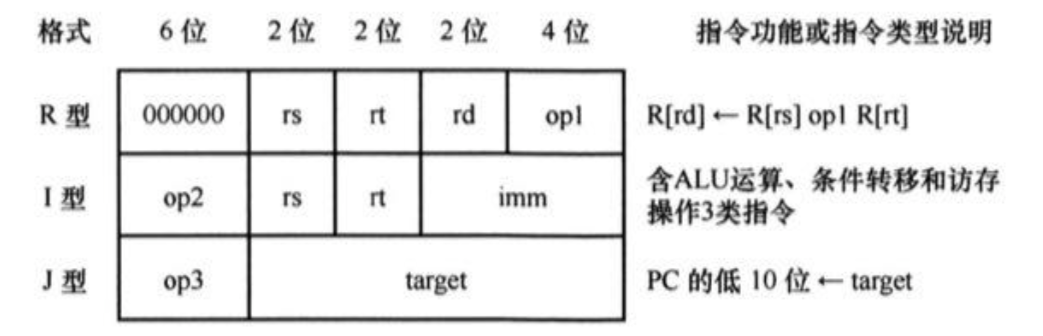
\includegraphics[width=10cm]{题目.png}
\end{figure}

其中,op1 $\sim$ op3 为操作码,rs,rt 和 rd 为通用寄存器编号,R[r] 表示寄存器 r 的内容,imm 为立即数,target 为转移目标的形式地址。回答以下问题:

\begin{enumerate}
    \item  ALU 的宽度是多少位?可寻址主存空间大小为多少字节?指令寄存器、主存地址寄存器(MAR)和主存数据寄存器(MDR)分别应有多少位?
    \item R 型格式最多可定义多少种操作?I 型和 J 型格式总共最多可定义多少种操作?通用寄存器最多有多少个?
    \item 假定op1为0010和0011时,分别表示带符号整数减法和带符号整数乘法指令,则指令01B2H的功能是什么(参考上述指令功能说明的格式进行描述)?若1、2、3号通用寄存器当前内容分别为B052H、0008H、0020H,则分别执行指令01B2H和01B3H后,3号通用寄存器内容各是什么?各自结果是否溢出?
    \item 若采用I型格式的访存指令中imm(偏移量)为带符号整数,则地址计算时应对imm进行零扩展还是符号扩展?
    \item 无条件转移指令可以采用上述哪种指令格式?
\end{enumerate}

}

\newpage
\backgroundsetup{contents=
\includegraphics{空白示例.png}, center, scale=1, angle=0, opacity=1}
\BgThispage
没见过那么长的题目,吓到了吗?别急,一题一题来。

\paragraph{【第 1 题】} 这题问的是各种「位数」的辨析。

题干表明按字节编址,并给出了四种「位数」:
\begin{itemize}[itemsep=0pt,parsep=0pt]
  \item 字长:16 位
  \item 地址线:20 位
  \item 数据线:8 位
  \item 指令字长:16 位
\end{itemize}
下面要问那么几个问题:
\begin{itemize}[itemsep=0pt,parsep=0pt]
  \item ALU 宽度:16 位——与字长相同,即为 ALU 运算对象的宽度;
  \item 可寻址主存空间大小:$2^{20}$ 字节(1 MB)——按字节编址,而且是 20 位地址线,因此存储芯片容量为 $1\mathrm{M}\times 8$ 位,即 1MB;
  \item 指令寄存器位数:16 位——与单条指令字长相同;
  \item 地址寄存器 MAR 位数:20 位——与地址线位数相同;
  \item 数据寄存器 MDR 位数:8 位——与数据线宽度相同。
\end{itemize}

\paragraph{【第 2 题】} 这题问的是指令系统,各种指令的可用数量。

\begin{figure}[htb]
    \centering
    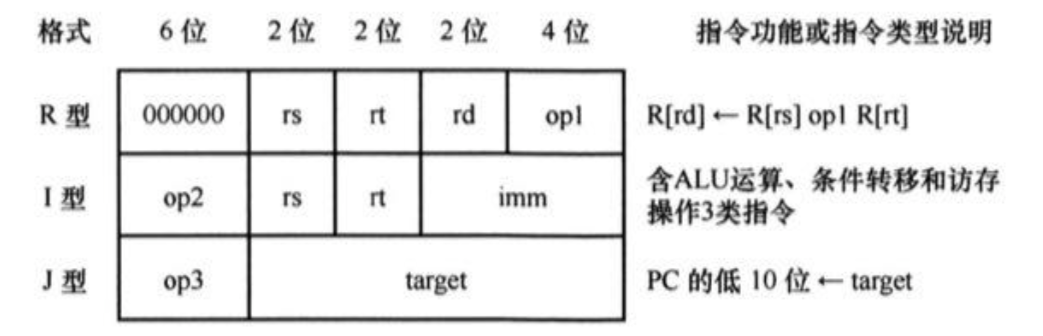
\includegraphics[width=10cm]{题目.png}
\end{figure}

\begin{itemize}
    \item R 型指令:这是三地址指令,op1 是 4 位操作码,所以共 $2^4=16$ 种。
    \item I,J 型指令:I 型是二地址指令,J 型是一地址指令,op2,op3 是 6 位操作码。本来能用 $2^6=64$ 种,不过全零的一种被 R 型指令占据,所以是 63 种。\textcolor{cyan}{注意题干问的是 I 型和 J 型格式「总共」可定义,这两种指令共享前 6 位的操作码空间。}
    \item 通用寄存器最多有多少个:寄存器编号 rs,rt,rd 都是 2 位,说明只有 00,01,10,11 共 4 种可能,因此最多有 4 个。
\end{itemize}

\paragraph{【第 3 题】} 这题问的是指令翻译,以及十六进制数的计算。

把两条指令都翻译一下,得到表 \ref{tab:instructions}:

\begin{table}[htb]
    \centering
    \begin{tabular}{cccccc}
    \toprule
    指令 & 二进制 & rs & rt & rd & op1 \\
    \midrule
    01B2H & 0000\ 0001\ 1011\ 0010 & 01 & 10 & 11 & 0010 \\
    01B3H & 0000\ 0001\ 1011\ 0011 & 01 & 10 & 11 & 0011 \\
    \bottomrule
    \end{tabular}
    \caption{第 3 题两条指令的信息}\label{tab:instructions}
\end{table}

\begin{figure}[htb]
    \centering
    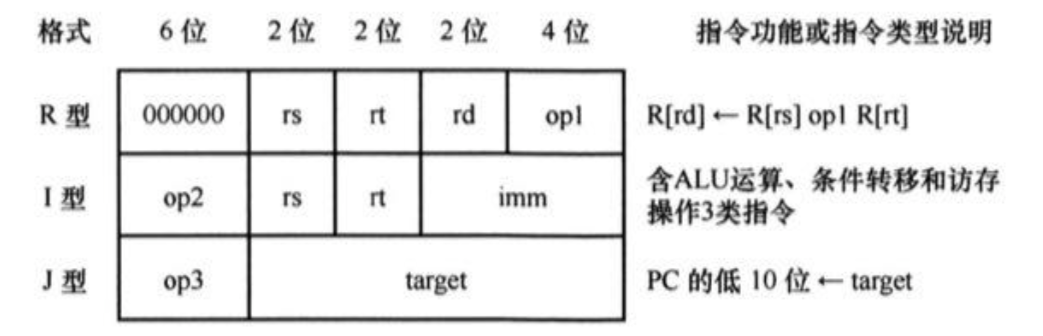
\includegraphics[width=10cm]{题目.png}
\end{figure}

于是指令 01B2H 的功能就是,把 1 号寄存器 rs 的内容和 2 号寄存器 rt 的内容做出带符号整数减法,放在 3 号寄存器 rd 中,也就是:$\mathrm{R[3] \gets R[1] - R[2]}$。

现在 R[1],R[2],R[3] 分别为B052H,0008H,0020H,执行指令 01B2H,列竖式计算:\textcolor{cyan}{(像三年级学过的四位数减四位数一样,最低位借来一个 16,作退位减法)}
\begin{table}[H]
  \centering
  \begin{tabular}{ccccc}
      & B & 0 & 5 & 2 \\
  $-$ & 0 & 0 & 0 & 8 \\
  \hline
      & B & 0 & 4 & A \\
  \end{tabular}
\end{table}
于是 R[3] 变成了 B04AH,没有溢出。

执行指令 01B3H,也就是 $\mathrm{R[3]\gets R[1]\times R[2]}$,也就是 $\mathrm{B052H\times 8}$。列竖式计算:
\begin{table}[H]
  \centering
  \begin{tabular}{crrrr}
           & B & 0 & 5 & 2 \\
  $\times$ & $_{\textcolor{green!50!black}{5}}$0 & 0 & $_{\textcolor{violet}{2}}$0 & $_{\textcolor{blue}{1}}$8 \\
  \hline
           & \textcolor{green!50!black}{8} & 2 & \textcolor{violet}{9} & \textcolor{blue}{0} \\
  \end{tabular}
\end{table}

\textcolor{cyan}{(在十六进制下:$2\times 8 = 16 = 10_{(16)}$,二八一十;$5\times 8 + 1= 41 = 29_{(16)}$,五八二十八,加一二十九;$\mathrm{B}\times 8 = 88 = 58_{(16)}$,B 八五十八。)}

于是 R[3] 变成了 8290H,而且有溢出(溢了一个 5)。

\begin{tcolorbox}[colback=violet!5, colframe=violet, boxrule=1pt, ]
\small
另一种理解方式是,把 B052H 左移 3 位,这样恰好是乘 $2^3$。
\begin{center}
    101\textcolor{violet}{1\ 0000\ 0101\ 0010} 
    
    \textcolor{violet}{1000\ 0010\ 1001\ 0}000 
\end{center}
由于 B052H 符号位为 1,是个负数,左移的时候移出了 101,并不都与符号位 1 相同,所以发生了溢出。或许这样理解更直观一些。

\end{tcolorbox}


\paragraph{【第 4 题】} 偏移量 imm 是带符号整数,相当于相对寻址的 S = ((PC)$\pm$ imm),所以当然带符号扩展。

\begin{tcolorbox}[colback=violet!5, colframe=violet, boxrule=1pt, ]
\small
零扩展和符号扩展:举个例子,要把一个 6 位二进制数扩展到 16 位,那么高 10 位应该填补 0 还是填补符号位?

比如数字 $6$:6 位二进制数为 000110,那么扩展后的 16 位数是 $\textcolor{violet}{0000\ 0000\ 00}00\ 0110$。此时零扩展和符号扩展都算正确。

比如数字 $-6$:6 位二进制数源码为 $100110$(最高位为符号),补码为 $111010$,那么扩展后的 16 位数应该是什么呢?

\begin{center}
    A. \textcolor{violet}{0000\ 0000\ 00}11\ 1010 \\
    B. \textcolor{violet}{1111\ 1111\ 11}11\ 1010
\end{center}
显然,A 属于零扩展,符号位在扩展后却消失了,明显不合适;B 属于符号扩展,填补了符号位 1,而且 B 还原至原码为 $1000\ 0000\ 0000\ 0110$,仍然是 $-6$。因此,\textbf{对于负数,只有符号扩展正确}。
\end{tcolorbox}

\paragraph{【第 5 题】} 无条件转移指令是 \verb!JMP x!,属于一地址指令,且需要更新PC内容,因此使用 J 型指令格式,把 target 写入 PC 的低 10 位,完成跳转。

\backgroundsetup{contents=
\includegraphics{下半示例.png}, center, scale=1, angle=0, opacity=1}
\BgThispage
\vspace{1em}
{\color{cyan!80!black}
【结论】见各题详细解析。

【点评】这道题是计组考研的一道综合题,融合了各种「位数」的辨析,指令系统中指令的类型、可用数量、指令翻译,十六进制数的运算,零扩展与符号扩展等知识点,难度较大,需要同学们把知识融会贯通才能解决此题。
}

\end{document}